In this chapter we wish to introduce different methods for modelling including hypothesis testing and cross-validation.
In addition, methods for validation of the models will be introduced and applied on the constructed models.

The chapter is based on \cite{Allison2012}, \cite{MadsenThyregod2011} and \cite{Wooldridge2012}.

\section{Modelling} \label{sec:modelling}
Based on the theory presented in chapter \ref{ch:Multip_linear_regresssion} we want to design a model and determine its coefficients. 
This will be done using the HOME dataset presented in chapter \ref{ch:introduction}. 
As argued there, the purpose is to predict prices based on selected independent variables that we suspect have an impact on the price of apartments in the selected cities.
The multiple regression model we will use in the following chapter is on the form
\begin{align*}
    \textit{price} &\sim \textit{cond} + \textit{size} + \textit{selling.period} + \textit{year.construct} + \textit{balcony} + \textit{renovation} + \textit{city} + \textit{year.sale}.
\end{align*}
%\begin{align*}
%    \textit{price} &\sim \beta_0 +  \beta_1\textit{cond} + \beta_2\textit{size} + \beta_3\textit{selling.period} + \beta_4\textit{year.construct}\\
%    &\qquad + \beta_5\textit{balcony} + \beta_6\textit{renovation} + \beta_7\textit{city} + \beta_8\textit{year.sale}
%\end{align*}
To justify the inclusion of these variables, their $R$-squared value will be determined. 
This method of excluding variabels is subjective, but gives an impression of how important each independent variables is to explaining the variability in the dependent variable \textit{price}. 
The table below contains the $R$-squared and adjusted $R$-squared for models with each of the independent variables respectively.
\begin{table}[H]
\centering
\footnotesize
\begin{tabular}{lrrrrrrrr}
\toprule
\textbf{}          & \textit{cond} & \textit{size} & \textit{selling.period} & \textit{year.construct} & \textit{balcony} & \textit{renovation} & \textit{city} & \textit{year.sale} \\
\midrule
$R^2$ & 0.001731                & 0.4862              & 7.514e-05           & 0.0001783                  & 0.02939        & 0.001312              & 0.3404   & 0.07557     \\
$R^2_{Adj}$ & 0.0010                & 0.4860              & 0.0002716           & -0.0001684                  & 0.0290        & 0.0009              & 0.3397  & 0.07493 \\
\bottomrule
\end{tabular}
\caption{\textit{R}-squared and adjusted \textit{R}-squared for the independent variables.}
\label{tab:r-squared}
\end{table}


Note that even if the $R$-squared is low, these parameters might still be significant and thereby improve the accuracy of the model, just not by much. 
The question is therefore rather if they are worth the added complexity.
We observe that with a tolerance level of 2 decimals, \textit{renovation}, \textit{selling.period} and \textit{year.construction} have coefficient of determination equal to zero and this may warant removing them from the model.

Categorical variables like \textit{city} are potentially problematic, as these are accounted for by dummy variables, that add a different intercept for the model depending on which city is observed.
In order for this to give an accurate estimate of the cities influence on price, the estimated coefficients for the other variables need to be similar for models made from data of the different cities. 
To illustrate this we have plotted \textit{price} against \textit{size} in figure \ref{fig:Forskellig_haeldning}, for each of the cities.
\begin{figure}[H]
    \centering
    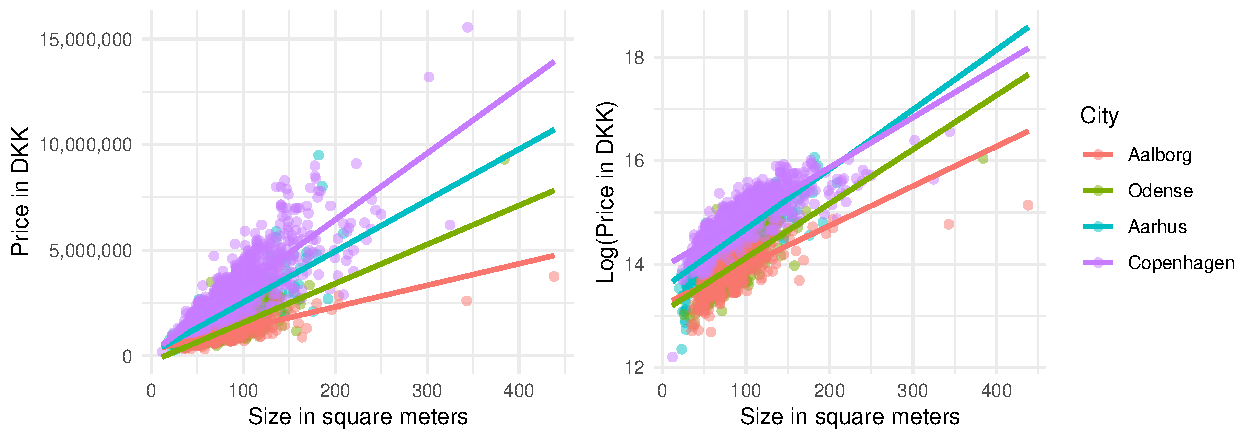
\includegraphics[width = 0.7\textwidth]{figures/Nanna/Forskellig_haeldning.pdf}
    \caption{The lines represents linear regressions where \textit{price} and $\log(price)$ is treated as the dependent variable and size in square meters the dependent variable.}
    \label{fig:Forskellig_haeldning}
\end{figure}
Making linear models for each of these groups, we find that the difference in slope between the models is significant.
For now this is simply seen from the figure \ref{fig:Forskellig_haeldning} and the coefficients in table \ref{tab:my-table}.
The term significance will be explored in more detail in section \ref{sec:Hypothesis_Testing}. 


\begin{table}[H]
\centering
\begin{tabular}{lrrrrrrr}
\toprule
\textbf{City}                                                                                       & \textbf{term}                & 
\textbf{estimate}            & \textbf{std.error}           & \textbf{statistic}           & \textbf{p.value}             \\
\midrule
Aarhus                                                                                & (Intercept)                  & 13.5                      & 0.0257                       & 527                         & 0                      \\
Aarhus                                                                            &  \textit{size}                   & 0.0115                       & 0.000325                         & 35.5                         & 1.24e-163                    \\
\addlinespace
Odense                                                                            &  (Intercept)                  & 13.1                     & 0.0310                       & 421                        & 0                    \\
Odense                                                                             &  \textit{size}                   & 0.0105                       & 0.000379                         & 27.7                        & 3.99e-105                    \\
\addlinespace
Aalborg                                                                           &  (Intercept)                  & 13.2                      & 0.0378                       & 350                         & 0                     \\
Aalborg                                                                            &  \textit{size}                   & 0.00766                       & 0.000425                         & 18.0                         & 1.14e- 53                    \\
\addlinespace
Copenhagen                                                                     &  (Intercept)                  & 13.9                      & 0.0196                       & 709.                        & 0                      \\
Copenhagen                                                                       &  \textit{size}                   &  0.00968                       & 0.000206                         & 47.1                        & 5.23e-273 \\                          
\bottomrule
\end{tabular}
\caption{Summary for the linear models $\log(price) \sim size$ in figure \ref{fig:Forskellig_haeldning}.}
\label{tab:my-table}
\end{table}

Adding \textit{city} as a parameter therefore decreases accuracy, and it might be wise to make separate models for each city. 
Note that this example only considers the size, and not the other categorical variables.

% Below in figure \ref{fig:Opfoerelsesaar_plot} is a plot of how the parameter \textit{year.construct} influences \textit{price}.
% As reflected by the $R$-squared value seen in table \ref{tab:r-squared}, \textit{price} varies significantly depending on \textit{year.construction}.
% We thereby conclude that this parameter is important and should be included in the model. 

% \begin{figure}[H]
%     \centering
%     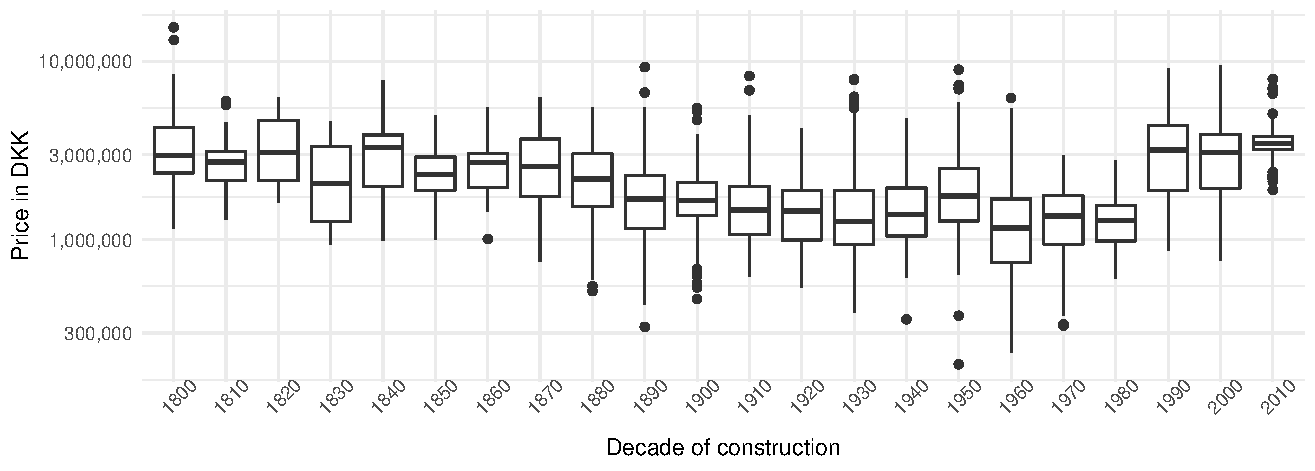
\includegraphics[width = 1\textwidth]{figures/Nanna/Opfoerelsesaarplot.pdf}
%     \caption{}
%     \label{fig:Opfoerelsesaar_plot}
% \end{figure}

From the left side of figure \ref{fig:Forskellig_haeldning} we see that the observations are heteroskedastic and their variance increases as \textit{size} increases. 
In order to satisfy the Gauss-Markov assumptions the observations need to have constant variance and we therefore need to transform the data, to remedy this. 
The logarithm is a variance stabilizing function, so using this on both \textit{price} and \textit{size} we see that the residuals seem to be approximately normally distributed around the regression line, as illustrated in figure \ref{fig:Log_Model_plot}. 

\begin{figure}[H] 
    \centering
    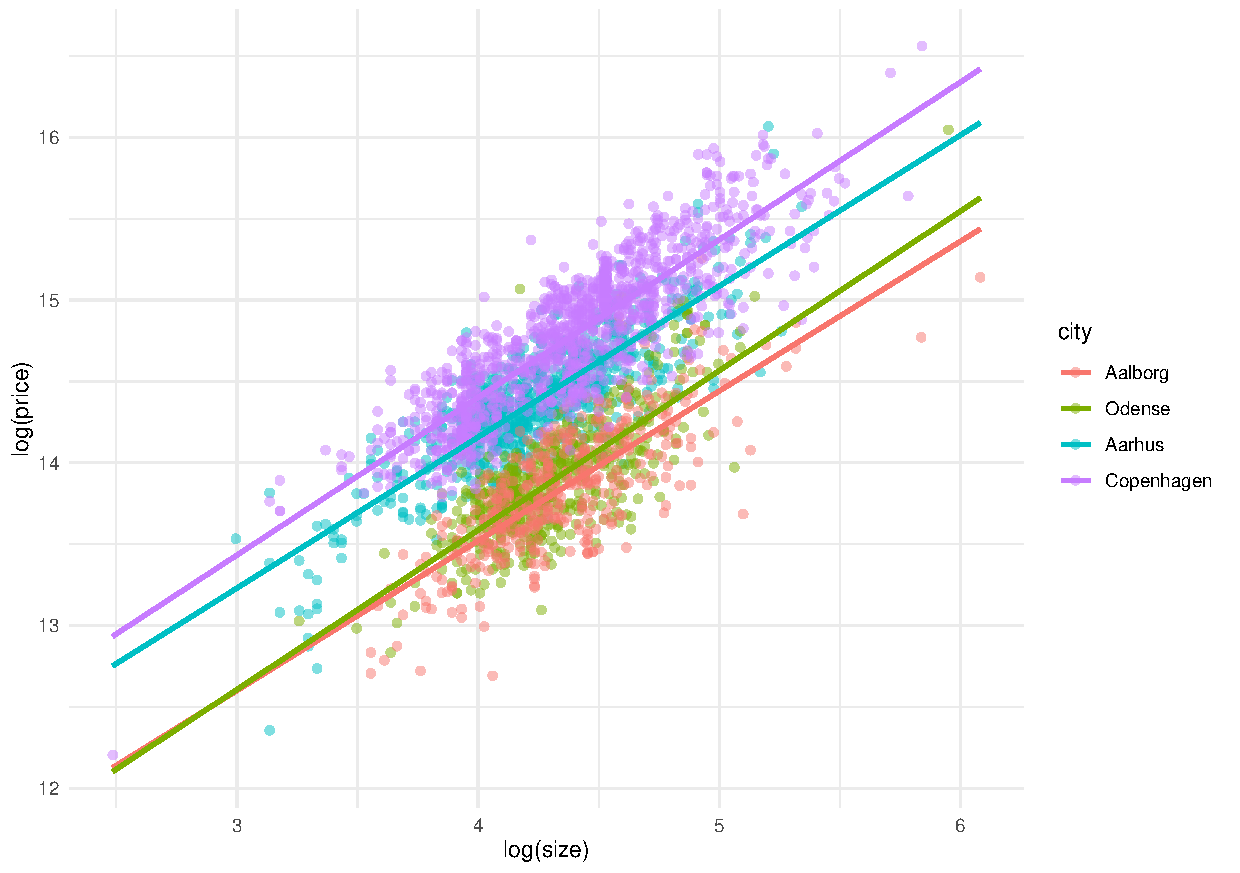
\includegraphics[width = 0.7\textwidth]{figures/Nanna/Plot_forskellig_haeldning.pdf}
    \caption{Simpel linear regression model with $log(price)$ as dependent variable and $log(size)$ as the independent variable.}
    \label{fig:Log_Model_plot}
\end{figure}

In the same manner we conclude, that the variance of the price is more homoskedastic after the log transformation, for all the independent variables listed in the model.
Now that the model has been separated into 4 models, one for each city, table \ref{tab:r-squared} is no longer valid.
The new models R-squared are presented in table \ref{tab:r-squared_4models}.

\begin{table}[H]
\centering
\footnotesize
\begin{tabular}{lrrrrrrrr}
\toprule
\textbf{}          & \textit{cond} & \textit{size} & \textit{selling.period} & \textit{year.construct} & \textit{balcony} & \textit{renovation}  & \textit{year.sale} \\
\midrule
$R^2_{Chp}$ & 0.112                & 0.6912              & 0.0007169           & 0.01179                  & 0.08983        & 0.01751      & 0.1021     \\
$R^2_{Aar}$ & 0.05409                & 0.6368              & 8.675e-05           & 0.009992                  & 0.05901        & 0.0006814        & 0.06073 \\
$R^2_{Ode}$ & 0.003955                & 0.6851              & 0.01061           & 0.02866                  & 0.004361        & 0.001168              & 0.003028 \\
$R^2_{Aal}$ & 0.003904                & 0.5104              & 0.001361           & 0.002269                  & 0.02415        & 0.003244              & 0.05763 \\
\bottomrule
\end{tabular}
\caption{\textit{R}-squared and adjusted \textit{R}-squared for the independent variables.}
\label{tab:r-squared_4models}
\end{table}
As predicted, the R-squared for size are larger, when splitting the model up into 4, allowing for better model fit.
Of note is the parameter $cond$ for Copenhagen, since this went from 0.001731 to 0.112, making it a much more useful parameter. 
Therefore we will use the following model as our full model, in the coming sections.
\begin{align*}
    \log(price) \sim \textit{cond} + \log(size)  + \textit{balcony} + year.sale.
\end{align*}

\subsection{Multicollinearity}
As it was explained in section \ref{sec:consequence_of_hetero} we desire as little multicolliearity as possible, as it increases the variance of the slope coefficients.
One way to quantify multicollinearity is
to use the variance inflation factor (VIF) which is defined as
\begin{align*}
    \text{VIF}_j = \frac{1}{1 - R^2_j}.
\end{align*}
The VIF can be interpreted as one of the three factors that inflates the variance of the slope coefficients, hence the name.
Performing regression for the 10 independent variables yield the VIF's displayed in table \ref{tbl:vif}.
\begin{table}[H]
    \centering
    \begin{tabular}{lrrrr}
        \toprule
        & \multicolumn{4}{c}{\textbf{VIF}} \\
        \midrule
        \textbf{Variable} & \textbf{Copenhagen} & \textbf{Aarhus} & \textbf{Odense} & \textbf{Aalborg} \\
        \midrule
        $\log(size)$                & 1.078182 & 1.067156 & 1.020253 & 1.022091 \\
        $balcony$                   & 1.167294 & 1.071244 & 1.010425 & 1.021054 \\
        $cond(medium)$              & 5.195332 & 9.506274 & 44.16799 & 11.06534 \\
        $cond(high)$                & 5.330074 & 9.586961 & 44.30732 & 11.02007 \\
        $year.sale(crisis)$         & 1.422332 & 1.275421 & 1.479368 & 1.287134 \\
        $year.sale(post.crisis)$    & 1.572893 & 1.308654 & 1.570689 & 1.264966 \\
        \bottomrule
    \end{tabular}
    \caption{VIF's for the variables in the model where a $year.sale(pre.crisis)$ and $cond(low)$ apartment is considered the baseline.}
    \label{tbl:vif}
\end{table}
Generally we have small values however for the dummy variables $cond(medium)$ and $cond(high)$ the VIF's are larger.
As suggested in \cite{Allison2012}, we can ignore high VIF's for dummy variables that represent a categorical variable with three or more categories.
These dummy variables will have high VIF's even though they are not associated with other variables in the regression model.
Thus we conclude that for all cities the VIF's for non dummy variables are at most 1.167294 which corresponds to an $R$-squared of approximately 0.143318, which we deem below our threshold for multicollinearity.
One should also be cautious how much weight is put on multicollinearity.
It is clear that other things equal we want lower multicollinearity as this will reduce the variance of the slope coefficients.
But multicollinearity, or VIF, is only one of three components in the slope coefficient variance.
The other two beign $\sigma^2$, the variance of the error term, and the total sample variation in $\textbf{x}_j$ given as $\text{SST}_j = \sum_{i=1}^n(\textbf{x}_{ij} - \overline{\textbf{x}}_j)$.